During the process of solving a MOKP or other multi-objective problems
one of the main general operation is to check if a solution is dominated
by another.
An algorithm may even require selecting all non-dominated solutions
from a large set of partial solutions.
This may demand quadratic effort on total number of solution if implemented
as pairwise comparison.
However, if solutions are mapped into points in a multi-dimensional space,
it can be deduced from equation~(\ref{eq:kdom}) that
this operation corresponds on checking whether a point exists in a certain region.
Formally:
\begin{align*}
    \text{ if } \; &\domk{y}{x} \; \text{ then } \; \pnt{y} \in R(\sol{x}) \\
  \text{where} \phantom{mmmmm} \\
    \pnt{x} &= \big(\obj{1}{x}, \ldots, \obj{\np}{x}, \weight{x}\big) \\
    R(\sol{x}) &= \left\{ a \in \mathbb{R}^{\np+1} \;\middle|\;
      a_{\np+1} \leq \weight{x}
      \, \text{ and } \,
      a_i \geq \obj{i}{x}, \; i \in \{1, \ldots, \np\}
      \right\}
\end{align*}

The problem of determining whether a point exists in a certain region
of space is known in geometric computation as
\emph{range search}~\cite{agarwal1999geometric}
and is usually solved with the use of a
\kdtree{}~\cite{preparata2012computational}.
The \kdtree{} is a type of binary search tree for indexing multi-dimensional
data with simple construction and low space usage.
Despite its simplicity, it efficiently supports nearest
neighbour search and range search operations~\cite{bentley1975} and
for those reasons \kdtree{} is widely used on
spacial geometry algorithms~\cite{preparata2012computational, guttman1984r},
clustering~\cite{kanungo2002efficient, indyk1998approximate}
and graphic rendering algorithms~\cite{owens2007survey}.

Like a standard binary search tree, the \kdtree{} subdivides data at each
recursive level of the tree.
Unlike a standard binary tree, that uses only one key for all levels of the tree,
the \kdtree{} uses $k$ keys and cycles through these keys for successive levels
of the tree.
Figure~\ref{fig:kdom-kd} presents
(a) points on a plane
indexed by a (b) \dtree{2}.
The first and third level of the \dtree{2} indexes $x$ component
while second level indexes $y$ component.
Each point branches a subregion in two -- showed on the figure by a
thicker line -- according to the component being indexed.

\begin{figure}[H]
  \centering
  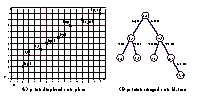
\includegraphics[scale=3.8]{img/kdt/dom-kd}
  \caption{Example of points indexed in a \kdtree{}.}
  \label{fig:kdom-kd}
\end{figure}

Figure~\ref{fig:query} presents an example of dominance check operation with indexed
solutions using a \dtree{2}.
The gray area has no intersection with the dominant (cross-hatched) area, therefore
solutions inside it are not evaluated.
The efficiency of this pruning action grows
with the amount of points.

\begin{figure}[H]
  \centering
  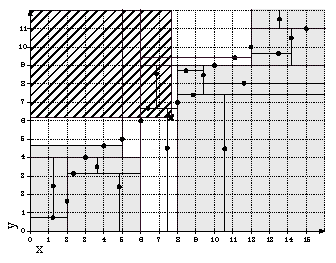
\includegraphics[scale=1.7]{img/kdt/query}
  \caption{Example of dominance check operation using \kdtree{} for solution indexing.}
  \label{fig:query}
\end{figure}

% Discussão sobre eficiencia da kdtree em relação ao número de dimensões:
Concerning the efficiency of the \kdtree{}, it is important to
consider the number of dimensions it is indexing.
As a general rule, a \kdtree{} is suitable for the efficiently indexing of $n$ elements
if $n$ is much greater than $2^k$.
Otherwise, when \kdtree{} is used with high-dimensional data, most of the elements
in the tree will be evaluated and the efficiency is no better than exhaustive search~\cite{toth2004handbook}.

It is expected that the use of a \kdtree{}
assists dominance check operation by
pruning a larger amount of points than a single dimensional indexing,
which may demand a smaller number of solution evaluation,
thus increasing algorithm performance.
The \kdtree{} can also be useful in the case of querying
solutions that are closest to a given one for which
a nearest neighbour search may be executed.
